%#BIBTEX pbibtex ComEX_template_v1_1
%% ComEX template ver1.0 June 22, 2012
%% ComEX template ver1.1 Sep. 23, 2014
%% ComEX template ver1.2 Sep. 10, 2019

%\documentclass[Proof]{comex}
\documentclass{comex}

\usepackage[dvips]{graphicx,color}
\usepackage{url}
\usepackage{algorithm}
\usepackage{algorithmic}

\vol{1}
\no{1} 

\title{Shadowing-Fading-based \\ Intersection  Geographic \\ Opportunistic Routing \\ Protocol   for Urban VANETs}

\author{Nobuyoshi Kikuma$^{\rm 1a)}$, Hiroyoshi Yamada$^{2}$,\\ and Kunio Sakakibara$^{1}$}
\affiliate{$^{1}$
Graduate School of Engineering, Nagoya Institute of Technology \\
Gokiso-cho, Showa-ku, Nagoya, Aichi 466-8555, Japan \\
$^{2}$ Faculty of Engineering, Niigata University \\
8050 Ikarashi 2-no-cho, Nishi-ku, Niigata 950-2181, Japan}

%Contact Person's E-mail Address.
\email{{\rm a)} kikuma@m.ieice.org}

\received{2012}{3}{00}
\accepted{2012}{3}{00}
%\published{2012}{1}{12}

\setcounter{page}{1}

\begin{document}

\maketitle

\begin{abstract}                                                                                                                                                                                                                                                                                                                                                                                                                                                                                                                                                                                                                                                                                                                                                                                                                                                                                                                                                                                                                                                                                                                                                                                                                                                                                                                                                                                                                                                                                                                                                                                                                                                                                                                                                                                                                                                                                                                                                                                                                                                      
Use this instruction file as a template for preparing your articles with
\LaTeX{} or Microsoft Word (MS Word). It is essential to adhere to this
template because your manuscripts are printed as submitted with minimal
editing/formatting by publisher. Do not modify any formats or
styles. Main text is limited to approximately 1,500 words, and abstract is about 100
words. You may include total maximum of three display items (figures, tables, algorithms, 
and so on) in principle but do not exceed 4 MB after converting to PDF.
Visit http://www.comex.ieice.org/ for the latest version of ComEX template.
\end{abstract}

\begin{keywords}
ComEX, template, comex.cls, up to six words
\end{keywords}

\begin{classification}
XYZ (choose one from the list in Sect.~\ref{sec:class})
\end{classification}

%%%%%%%%%%%%%%%%%%%%%%%%%%%%%%%%%%%%%%%%%%%%%%%%%%%%%%%%%%%%%%%%%%%%%%%%
%% For bibtex users:
%\bibliographystyle{comex} % Bibtex style file for ComEX
%\bibliography{mybib} % Sample bibtex source file
%% These bibtex files are contributed by Dr. Ryutaro Matsumoto
%%%%%%%%%%%%%%%%%%%%%%%%%%%%%%%%%%%%%%%%%%%%%%%%%%%%%%%%%%%%%%%%%%%%%%%%

\begin{thebibliography}{1} \providecommand{\urlstyle}[1]{} \urlstyle{rm}

\bibitem{web_link}
{Editorial Committee of ComEX}, ``Information for the {IEICE} communications
  express (comex) authors, preparing manuscript,'' Institute of Electronics,
  Information and Communication Engineers,
  \url{http://www.comex.ieice.org/data/for_authors.html#preparing}, accessed
  Sep. 23, 2014.

\bibitem{journal_paper}
A.~B. Author1, C.~D. Author2, and E.~F. Author3, ``Title of journal paper with
  a comma inside the quotation marks like this,'' {\em Journal Title in
  Italic}, vol.~12, no.~3, pp.~456--789, month\ year.
\newblock \url{DOI:XX.XXXX/XXXXX}

\bibitem{chapter}
A.~B. Chapter-Writer, ``Title of quoted chapter,'' in {\it Book Title in Italic
  without Quotation Marks}, ed.~C.~D. Editor, pp.~123--456, Publisher Name,
  City, year.
\newblock \url{DOI:XX.XXXX/XXXXX}

\bibitem{book}
A.~B. Book-Author, {\em Book Title in Italic without Quotation Marks},
  Publisher Name, City, year.
\newblock \url{DOI:XX.XXXX/XXXXX}

\bibitem{proceeding_paper}
A.~B. Author1, C.~D. Author2, and E.~F. Author3, ``Title of paper in
  proceeding,'' Proc. 12$^{\mathrm{th}}$ Conf. Name, City, Country,
  pp.~123--345, PAPER-ID, month\ year.
\newblock \url{DOI:XX.XXXX/XXXXX}

\end{thebibliography}\urlstyle{tt}


\section{Introduction}

This template provides formats and styles for ComEX manuscript. It is
essential to adhere to this template because your manuscript will be
published ``{\it as is}'' with minimal copy-editing by the publisher. Do
not modify formats (font, font size, paper size, printing area, line
space, etc.).  {\it Keep one copy of this template untouched for your
reference and prepare your manuscript on another copy.}

\section{Software and article charge}

MS Word and \LaTeX{} compatible files are officially acceptable for
ComEX submission. These template files are designed for MS Word. \LaTeX{}
style files can be found elsewhere \cite{web_link}.  
Article charge is JPY~41,905 for a manuscript 
using MS Word template and JPY~31,429
for a manuscript using \LaTeX{} style file. 
Supplementary movie file(s) costs extra JPY 3,666 per movie file.

\section{Manuscript length}

Papers do not usually exceed six (6) pages of an A4-sized PDF file. The
first page contains paper title, author list, affiliation(s),
100-word-abstract, keywords, and references.  The main body of the text
is limited to approximately 1,500 words. Manuscripts are allowed to have
up to three (3) display items (Figures and/or Tables) with brief
captions in principle as long as the final PDF file size would not
exceed 4 MB. 

\section{Typographical style}

Consult with Table~\ref{tab:style} on the detail typographical styles.

\begin{table}[ht]
\begin{center}
\caption{ComEX typographical style} \label{tab:style}
\begin{small}
\begin{tabular}{lcl}
\hline
Article title & \quad &  Arial 26pt Bold Green\\
\hline
Author Name & \quad & Times New Roman 12pt Bold Black\\
\hline
Author Affiliation & \quad & Times New Roman 10pt Italic Black\\
\hline
Author Address & \quad & Times New Roman 10pt Italic Black\\
\hline
Author Contact E-mail & \quad & Times New Roman 10pt Italic Blue\\
\hline
Section Heading & \quad & Arial 11pt Bold Black\\
(incl. ``Abstract'' and ``Keywords'') & & \\
\hline
Abstract Body & \quad & Times New Roman 11pt Black\\
\hline
Reference Body & \quad & Times New Roman 10pt Black\\
\hline
Section Title & \quad & Arial 12pt Bold Black\\
\hline
Text Body & \quad & Times New Roman 11pt Black\\
\hline
Figure \& Table Label in Caption & \quad & Times New Roman 10pt Bold Black\\
\hline
Figure \& Table Caption Body & \quad & Times New Roman 10pt Black\\
\hline
Acknowledgment Body & \quad & Times New Roman 11pt Black\\
\hline
\end{tabular}
\end{small}
\end{center}
\end{table}


\subsection{Title}

Title should start flush left. Only the first letter in the title is
capitalized (this is true to section titles and figure captions).
Avoid including abbreviations unless definitely needed.

\subsection{Author name and affiliation}

Author names should start flush left. Spell out both first and last
names but initial middle name. Use one blank line between authors from
different affiliations.

\subsection{Abstract}

The abstract should be complete sentence(s) that is limited to
approximately 100 words. It should be a concise summary of the paper
that clearly conveys
problem,
methods, and
conclusions to readers. It also should include appropriate keywords for
the convenience of computer search. Do not include reference numbers.

\subsection{Keywords}

Maximum six (6) keywords are listed. Carefully choose appropriate
keywords for your paper being correctly spotted by the computerized search.

\subsection{Classification}
\label{sec:class}
Category index in the classification is used by the Editors 
when directing your manuscript to corresponding Associate
Editor. Furthermore, it is displayed in ComEX website and in archives for
readers' convenience. Choose the most relevant category from
the list below.

\begin{itemize}
\begin{small}
\item Fundamental theories for communications 
\item Energy in electronics communications 
\item Transmission systems and transmission equipment for communications
\item Optical fiber for communications
\item Fiber-optic transmission for communications
\item Network system
\item Network
\item Internet
\item Network management/operation
\item Antennas and propagation
\item Electromagnetic compatibility (EMC)
\item Wireless communication technologies
\item Terrestrial wireless communication/broadcasting technologies
\item Satellite communications
\item Sensing
\item Navigation, guidance and control systems
\item Space utilization systems for communications
\item Multimedia systems for communications
\end{small}
\end{itemize}

The Editorial Committee may change the
subject index that authors select if the Editorial Committee judges
that the authors' selection is not the best.  Note that the index might
be changed without notification.


\subsection{Main text and headings}

Single column format is applied throughout the manuscript. The first
line of the first paragraph of each section start flush left. Section
headings are numbered consecutively in Arabic numbers. Subsection
headings are numbered in Arabic numbers to the right of the decimal
point (like this 4.5).

\subsection{Equations}

Equations are centered with the equation number (in Arabic) appearing at
the right-hand margin, in parenthesis:
\begin{equation}
T_{\mbox{M}}^{\phi} = 2 \times \frac{G w t^3}{3 l} \phi \left( 1 - \frac{192}{\pi^5} {\frac{t}{w}} \tanh \frac{\pi w}{2 t} \right).
\label{eq:T_M^phi}
\end{equation}
\noindent
%
Long equations can be folded in several lines but avoid leading to
misinterpretation. Equations are referenced in the main text as
Eq.~(\ref{eq:T_M^phi}).


\subsection{References}

References should appear on the first page of the paper, in the order in
which they are referred in the main text. See the example in this
template for different styles for citing a journal paper, a whole book,
a contributed chapter in a book and a proceeding paper. WWW links can be
placed as a reference. It is authors' responsibility to provide correct
information of references. Use a pair of square bracket to cite
reference like [2]. Multiple references can be cited like~\cite{journal_paper,chapter,book,proceeding_paper}.

Note that refereed materials such as proceedings of international conferences should be cited in 
submitted material as the footnotes or references. 
In addition, authors are required to clearly indicate how the submitted material differs from the 
prior refereed works in Introduction. 
An example of sentences in Introduction and footnote is shown below:

This letter, which was previously presented at IEICE APCC 2019 [5]\footnote{In this letter, the impact of packet loss is newly considered.}, 
presents a novel MAC protocol of $\ldots$


\subsection{Acknowledgments}

Acknowledgments, if any, can be placed at the end of the manuscript.

\section{Display items (figures, tables, algorithms, and so on)}

You may include total maximum three (3) pieces of display items in
principle in a final PDF version of your manuscript but do not exceed 4 MB file size.



\subsection{Figures}

Figures should be placed in the document.  Do not submit figures in
separate files.  For \LaTeX{} users, use \LaTeX{} environment ``figure'' (\verb+\begin{figure}-+\linebreak
%%%%%%%%%%%%%%%%%%%%%%%%%%%%%%%%
\verb+\end{figure}+) to
place frames for figures. Place your figure as close to as the main text
where it is referred.  Figure position in the published paper may differ
from that in your original file, when publisher adjusts the final
format. Figures are numbered in Arabic numerals. Figures are referred as
Fig.~\ref{fig:scanner} even at the beginning of a sentence. Figure
captions are placed under corresponding figures.

\begin{figure}[htb]
\begin{center}
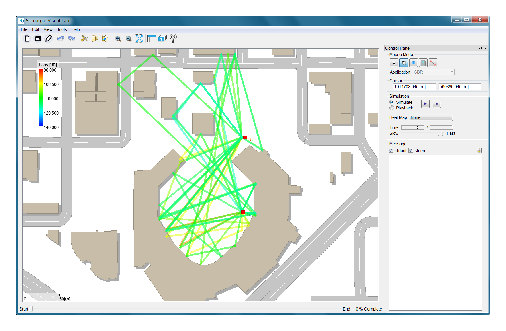
\includegraphics{f01.eps}
\end{center}
\caption{Include all graphics in the manuscript file. Do not submit
figures in separate files.}  \label{fig:scanner}
\end{figure}

\subsection{Tables}

Tables are placed in the document in the same manner as figures. Tables
are referred in Roman numbers such as Table~\ref{tab:style}, without
abbreviating to Tab.~\ref{tab:style}. Table captions are placed above
the corresponding tables.

\subsection{Algorithms}
If an algorithm or a pseudo code are shown in the form as Algorithm~\ref{alg1} below,
it is regarded as one of three display items allowed to be included in the final manuscript.
 
\begin{algorithm}[h]
\caption{Calculate $y = x^3$}
\label{alg1}
\begin{algorithmic}
\REQUIRE $x$
\ENSURE $y = x^3$
\STATE $y \Leftarrow x \times x$
\STATE $y \Leftarrow y \times x$
\end{algorithmic}
\end{algorithm}

\section{Supplementary Movies}

You can submit supplementary movies which will be placed on J-STAGE with your article.
General movie files such as Moving Picture Experts
Group (MPEG) format file or MOV format file are acceptable for movies.

\section{ORCID (Open Researcher and Contributor ID)}

Authors who would like to include their Open Researcher and Contributor ID (ORCID) in the
 published manuscript are required to upload a text file named "ORCID.txt" including 
 the list of name and ORCID of each author in the following format:\\
Name of author 1, ORCID of author 1\\
Name of author 2, ORCID of author 2\\
...\\
Note that ORCID will not be included in advanced publication articles.

\section{Conclusion}

To submit your manuscript to ComEX, visit an IEICE website \\
\verb+(https://review.ieice.org/regist_elex_e.aspx?cmdtype=ComEX)+ \\
to complete a Submission Form and to upload the following items: a PDF
file for review; an electronic file of manuscript in either \LaTeX{} or
MS Word; original artwork in separate electronic files. 
Art-file formats are restricted. Only the Encapsulated PostScript
(EPS) format file is allowed for graphics. 
If you submit supplementary movies, contact the IEICE Publishing Office (comex@ieice.org). 
Self-descriptive file names such as fig1.eps and fig2.mpg are preferred.
Authors are also requested to
select the subject index (code and field) best fitting manuscript from
the candidates. The index is used by the Editors when
directing manuscript to corresponding Associate Editor. Furthermore, it
is displayed in ComEX website and in archives for readers'
convenience. The Editorial Committee may change the subject index that
authors select, if the Editorial Committee judges that the authors'
selection is not the best.

\section*{Acknowledgments}

Your acknowledgments to co-workers and financial sponsors are placed here.

\end{document}
